\section{多电子原子: 泡利原理}
\subsection{泡利(Pauli)不相容原理}
原子中每个状态只能容纳一个电子. 

\textbf{费米子(如电子)满足泡利不相容原理, 而玻色子(如光子)与泡利不相容原理无关. }

\section{X射线}
\subsection{莫塞雷(Moseley)实验}
用电子轰击不同的材料, 得到不同的X谱线. 
\begin{figure}[!htb]
\centering
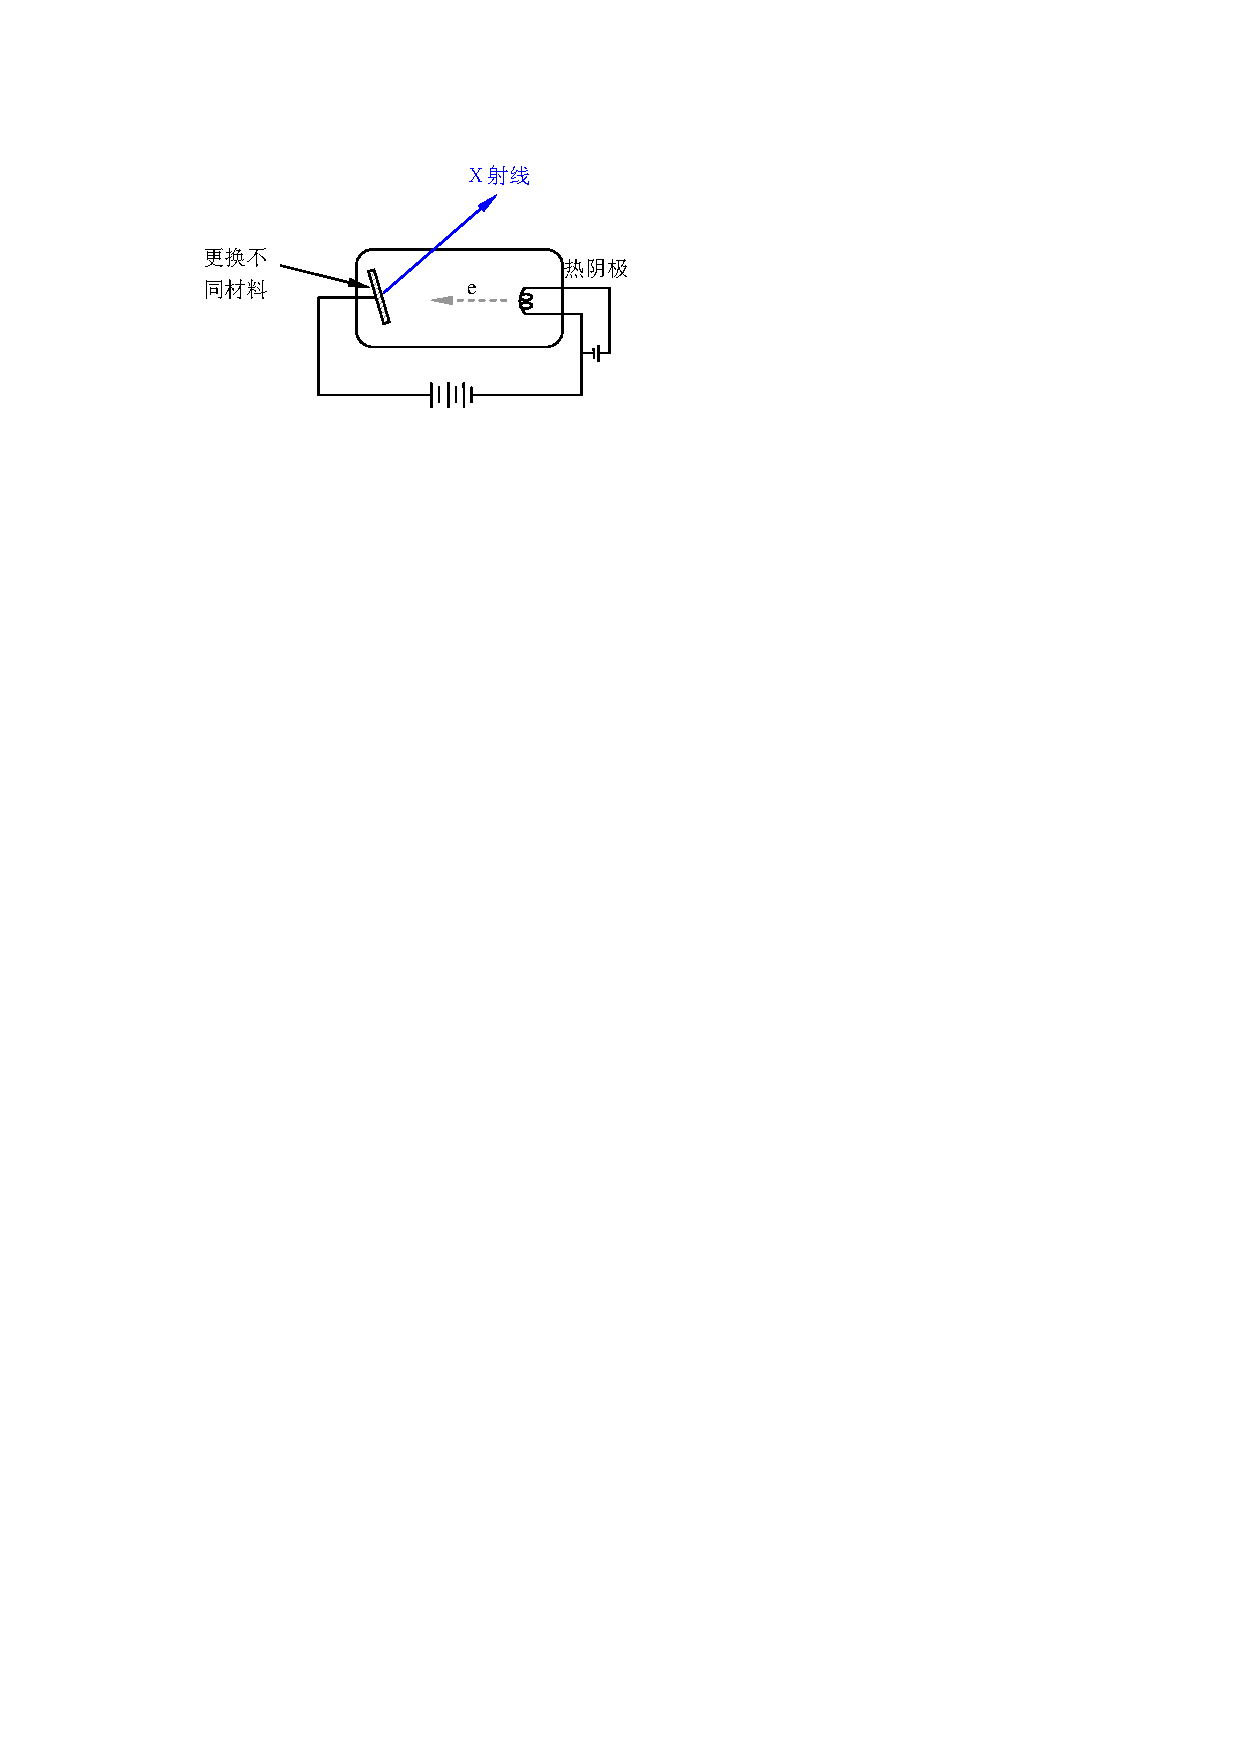
\includegraphics[width=0.5\textwidth]{fig10.pdf}
\caption{\label{fig10}莫塞雷(Moseley)实验}
\end{figure}

方法: 纵轴上用的是X相对强度, 这样能更清楚的区别不同材料的X光谱. 

结论: $\sqrt{\nu}\varpropto Z$(原子序数), 反应近原子核电子状态信息

应用: 元素周期表, 相近原子量的物质区分(如金和铂的区分). 

\subsection{朗伯-比耳(Lambert-Beer)定律}
\begin{figure}[!htb]
\begin{minipage}[b]{0.48\textwidth}
\centering
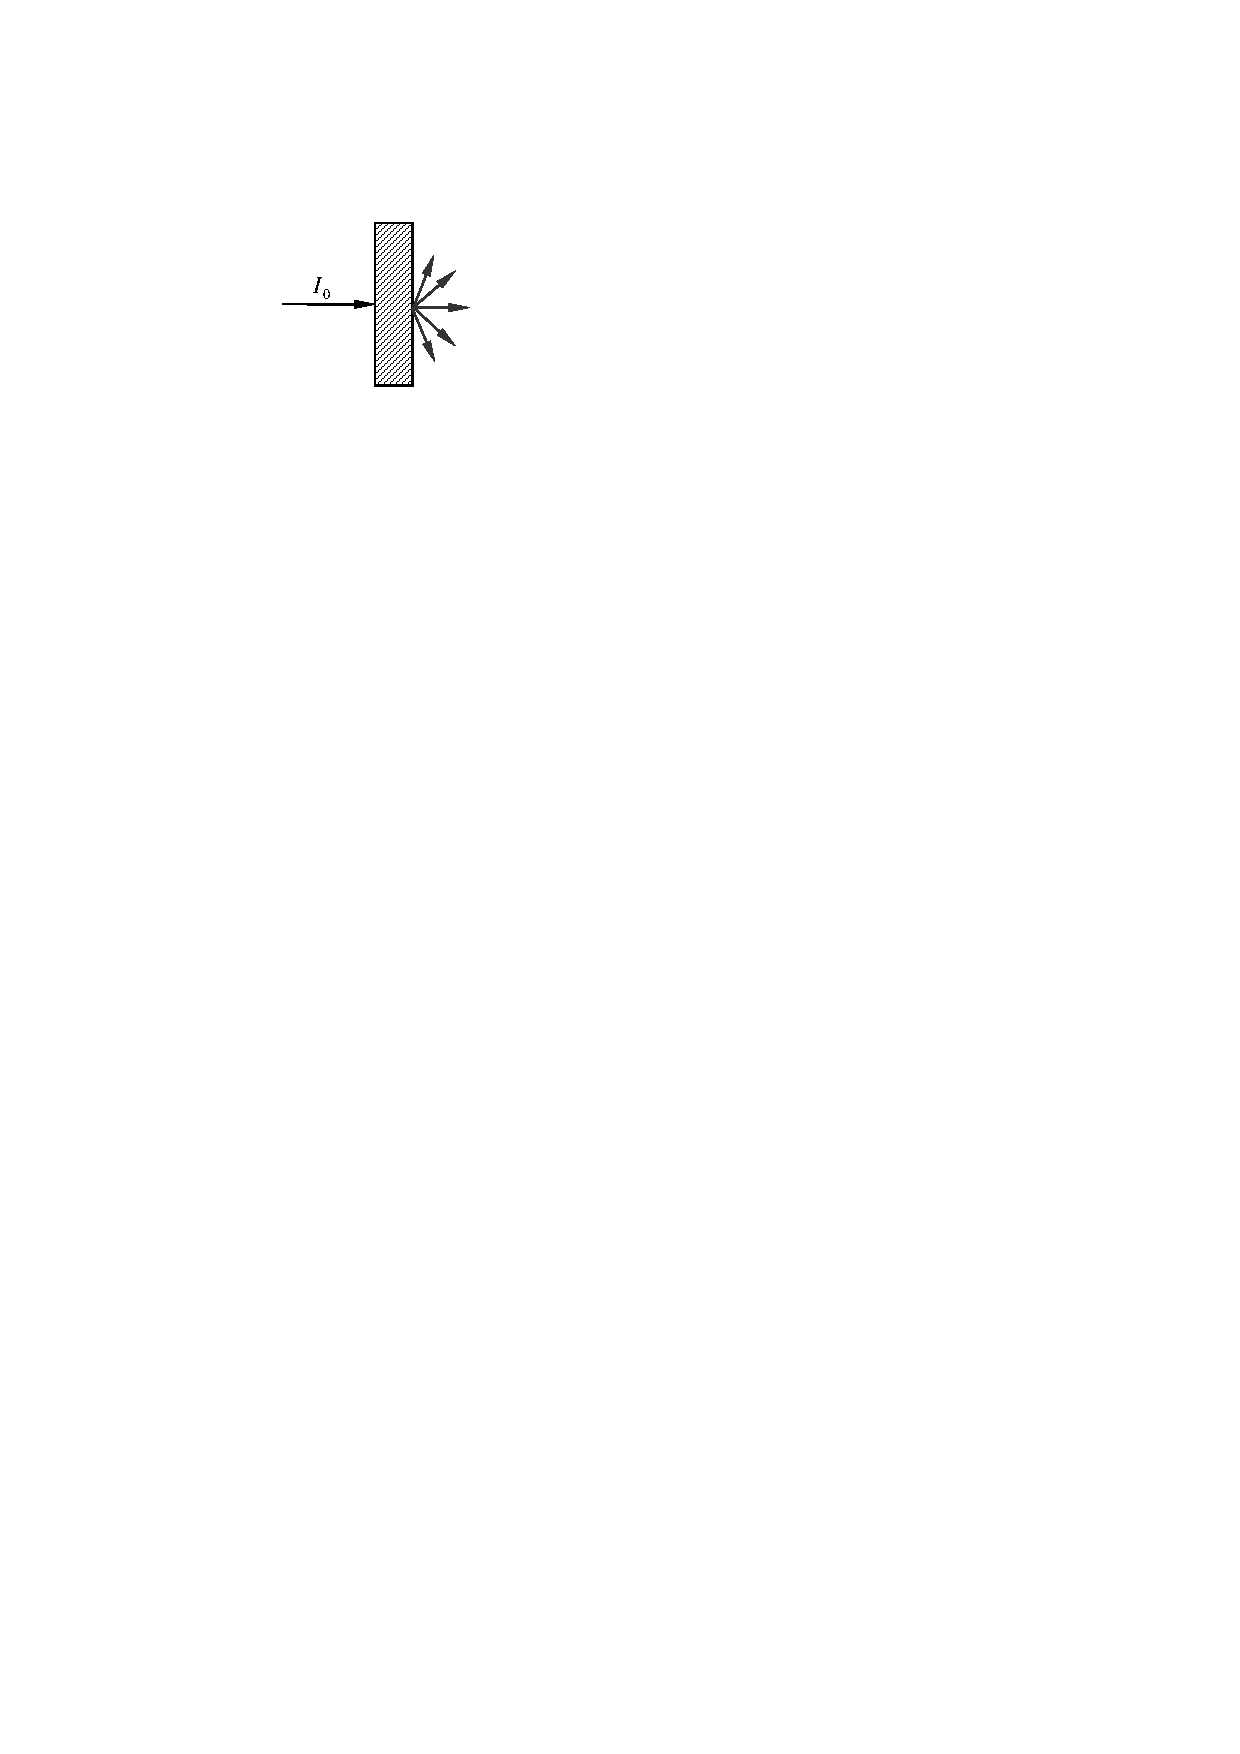
\includegraphics[width=0.5\textwidth]{fig12.pdf}
\caption{\label{fig12}粒子穿过材料}
\end{minipage}%
\begin{minipage}[b]{0.48\textwidth}
\centering
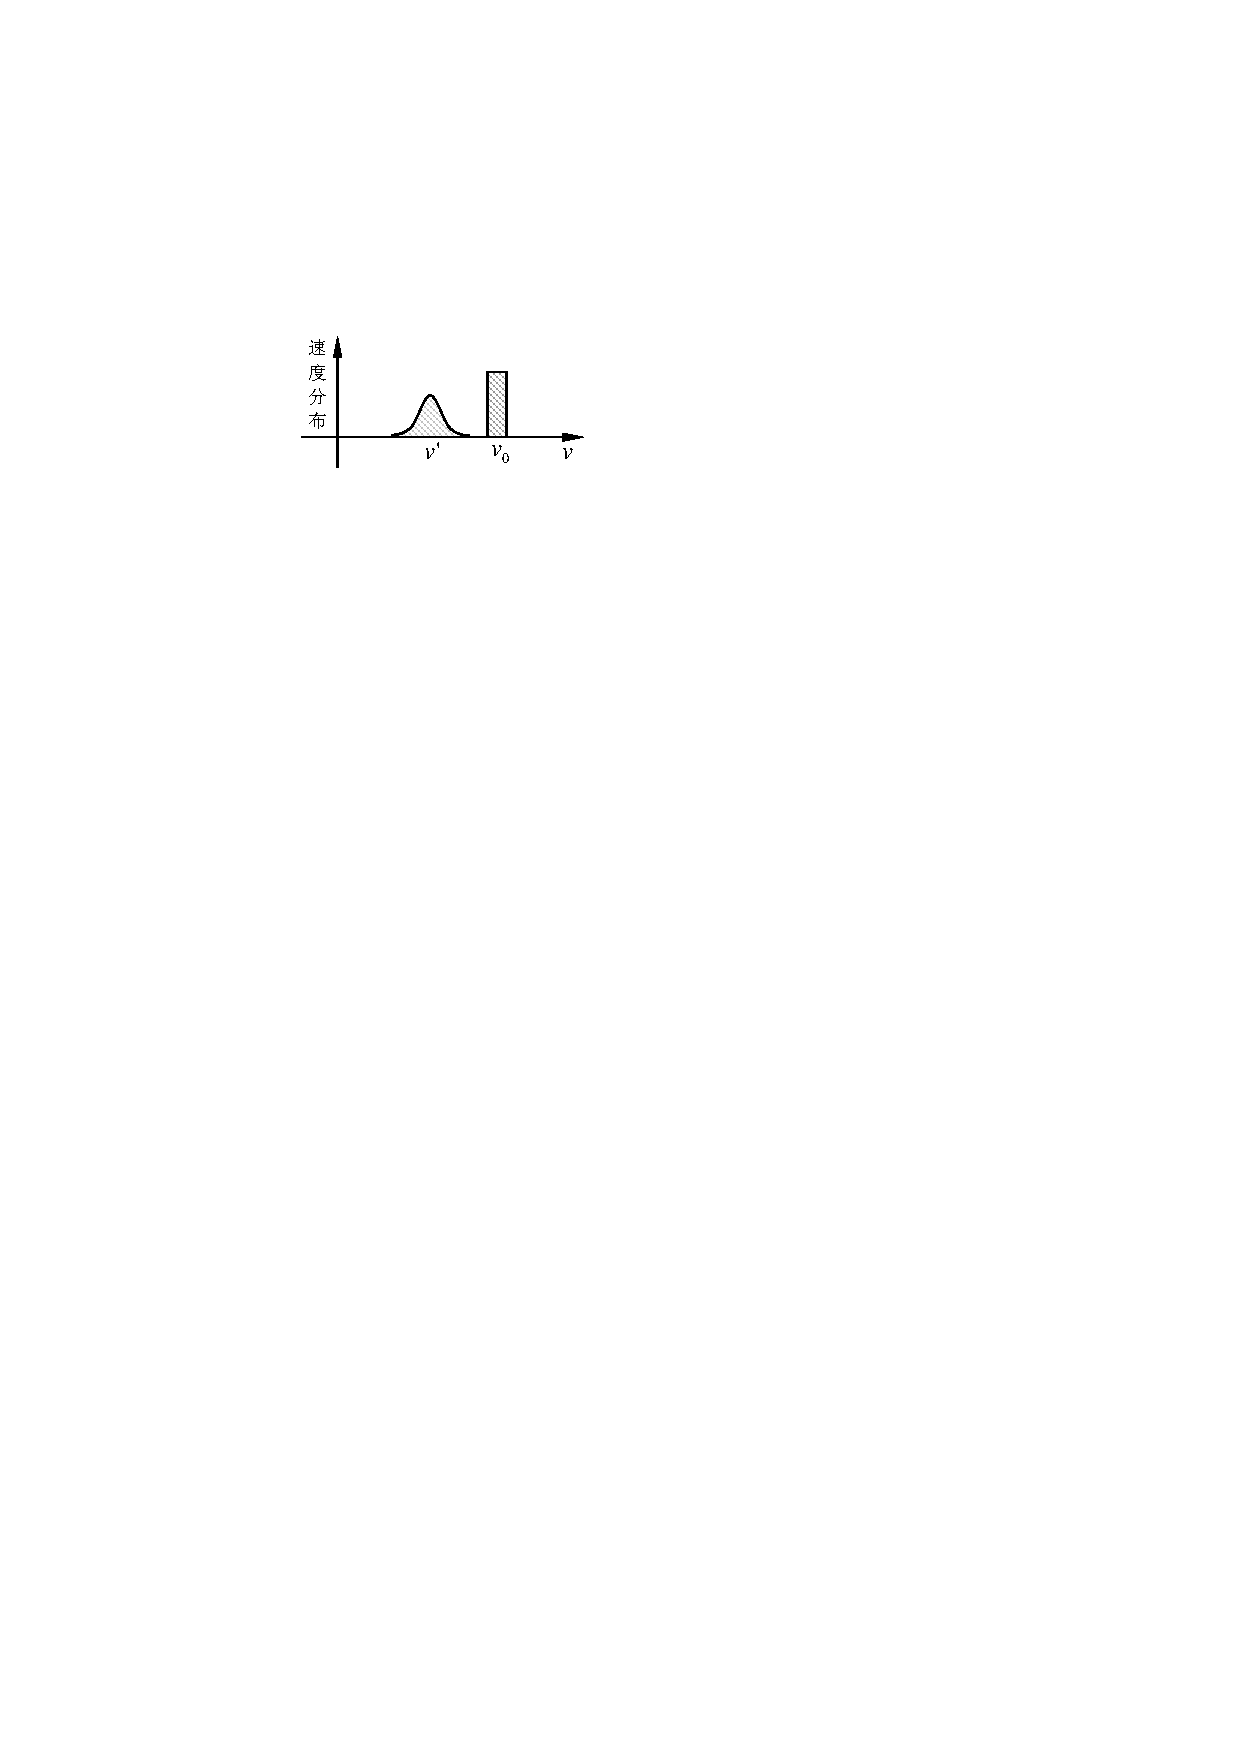
\includegraphics[width=0.6\textwidth]{fig13.pdf}
\caption{\label{fig13}出速粒子的速度分布}
\end{minipage}
\end{figure}
一束粒子强度为$I_0$, 通过厚度为$\textrm{d}x$的吸收体后, 强度必然减少, 减少量$\textrm{d}I$显然正比于厚度$\textrm{d}x$, 也正比于束流的强度$I$, 若把比例常数记为$\mu$, 则有
\[
-\textrm{d}I=\mu I(x)\textrm{d}x
\]
积分后得到
\[
I=I_0e^{-\mu x}
\]
这就是朗伯-比耳(Lambert-Beer)定律, 它不仅适用于粒子, 也适用于波(当然, 用于波时, 图\ref{fig13}将不再表示波的速度, 而表示波的频率). 

\noindent[\textbf{思考}]: 对于速度分布为图\ref{fig13}出射粒子, 其德布罗意波长分布是怎样的?电子的衍射实验能证明衍射图案是电子直接产生的吗, 能证明粒子的波动性吗, 为什么?

\subsection{康普顿(Compton)散射}
\begin{figure}[!htb]
\centering
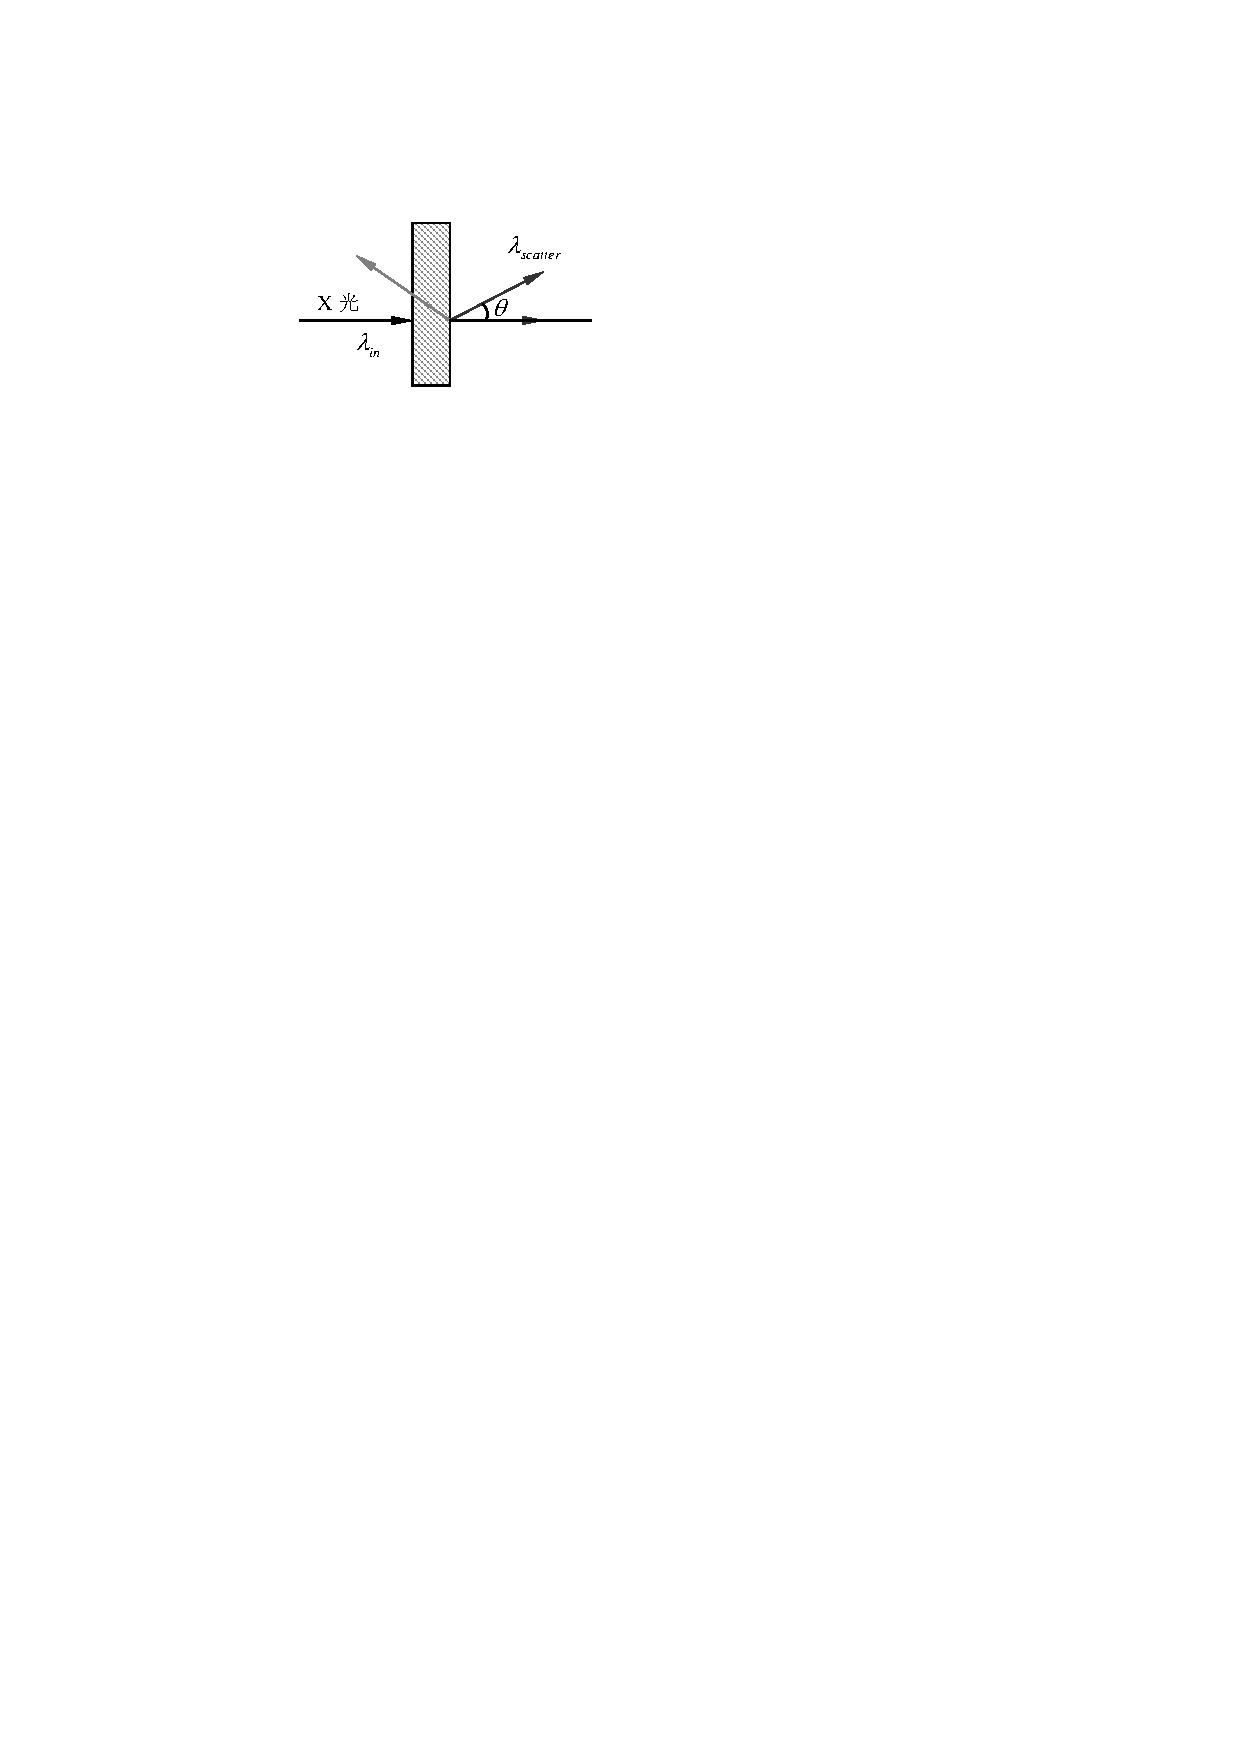
\includegraphics[width=0.35\textwidth]{fig11.pdf}
\caption{\label{fig11}康普顿散射}
\end{figure}
用X光照射晶体材料, 入射$\lambda_{in}$与出射$\lambda_{Scatter}$有以下关系: 
\[
\Delta\lambda=\lambda_{scatter}-\lambda_{in}=2k\sin^2\frac{\theta}{2}
\]
$k$是常数, 实验测得. 当换材料时, 公式不变, 即散射结果与材料无关. 揭示: 反映原子外层电子信息. 

\subsection{其它散射}
\begin{itemize}
\item \textbf{锐利散射}: 入射光在线度小于光波长的微粒上散射后散射光和入射光波长相同. 
\[
I_{sc}\propto\frac{k}{\lambda^4}
\]
正午时, 太阳直射地球表面, 太阳光在穿过大气层时, 各种波长的光都要受到空气的散射, 其中波长较长的波散射较小, 大部分传播到地面上. 而波长较短的蓝, 紫光, 受到空气散射较强, 但是人对紫光不敏感. 天空中的蓝色正是这些散射光的颜色, 因此天空会呈现蓝色. 
\begin{figure}[!htb]
\centering
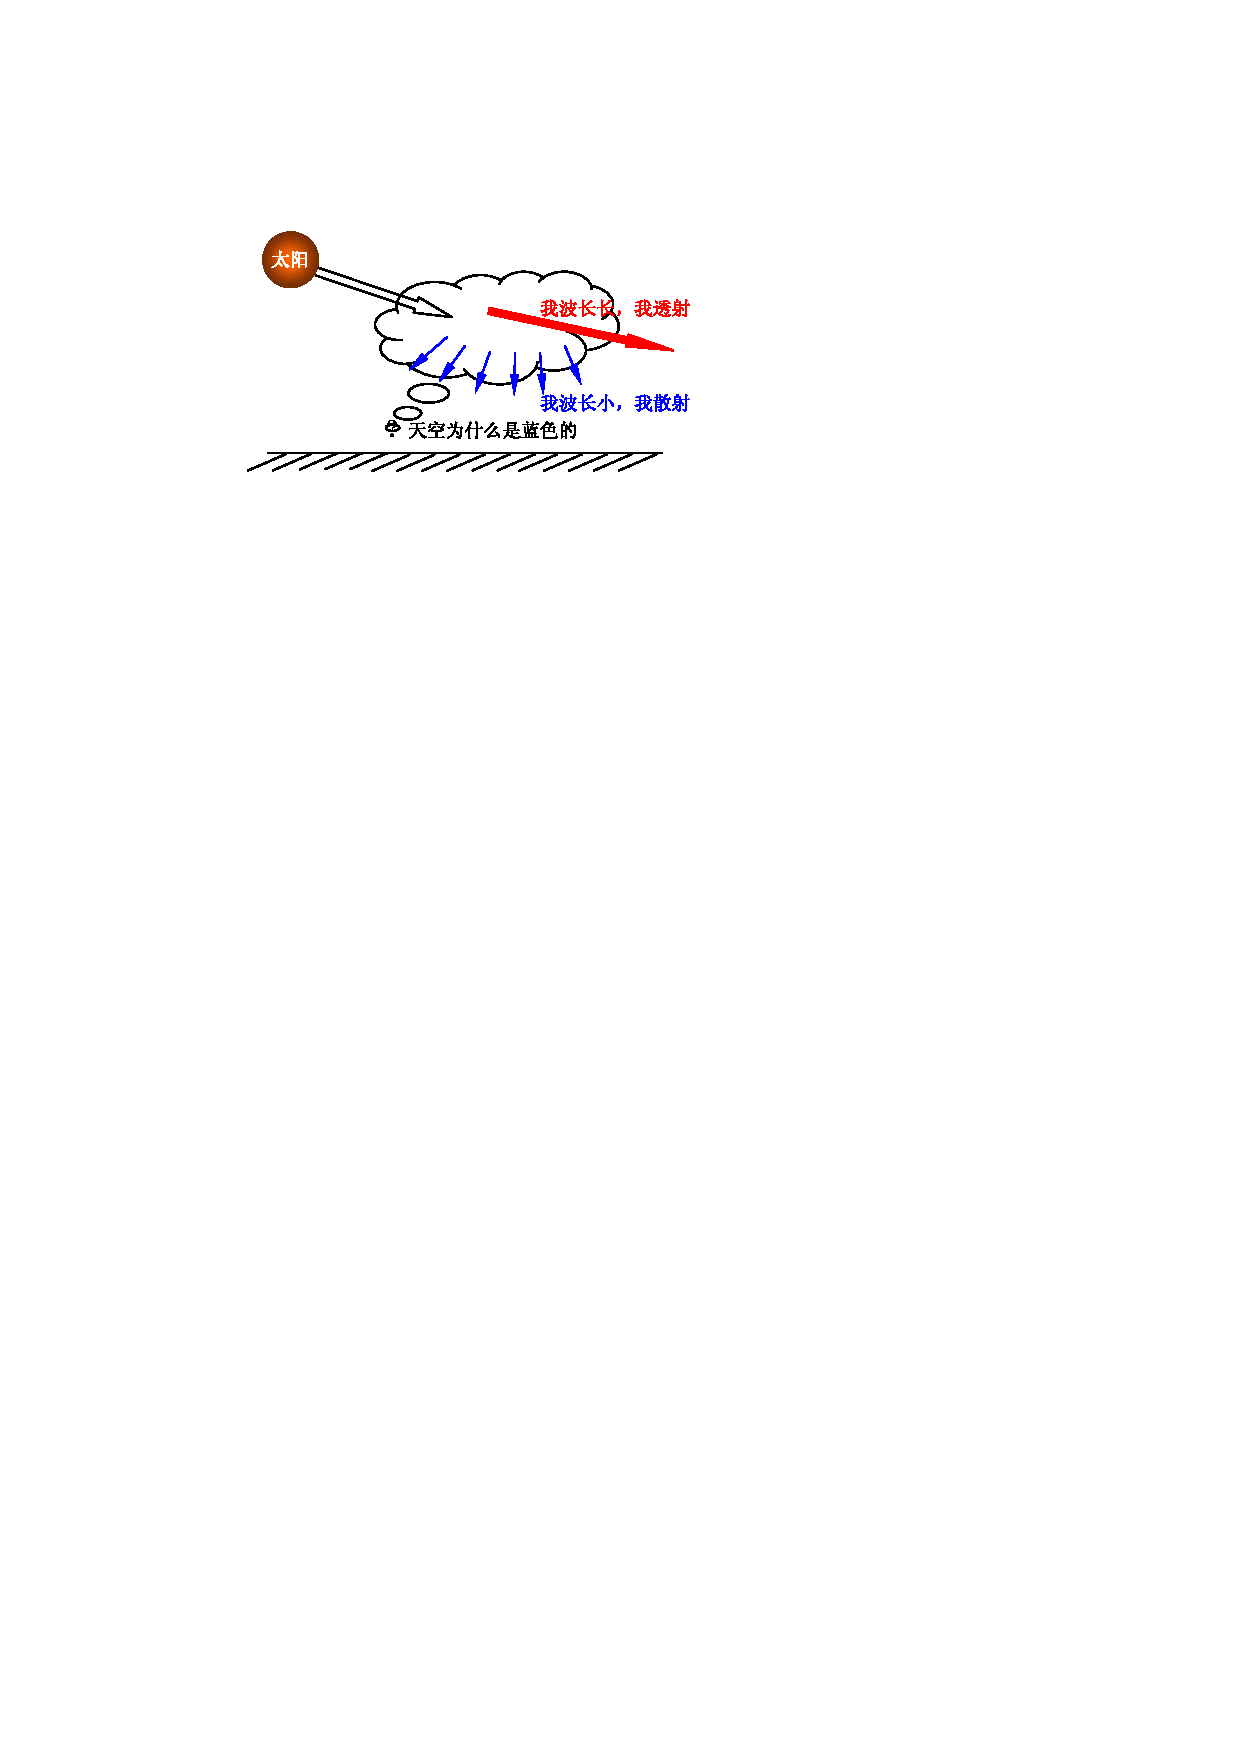
\includegraphics[width=0.5\textwidth]{fig17.pdf}
\caption{天空为什么是蓝色?}
\end{figure}

\item \textbf{拉曼散射}: 光通过介质时由于入射光与分子运动相互作用而引起的频率发生变化的散射.  拉曼散射也有$\Delta\lambda=\lambda_{sctter}-\lambda_{in}$, 但没有康普顿散射. 拉曼散射一般用紫外光, 而紫外光尺度大于原子, 只能反应分子的相互作用信息. 
\end{itemize}


